% Latex template: mahmoud.s.fahmy@students.kasralainy.edu.eg
% For more details: https://www.sharelatex.com/learn/Beamer

\documentclass{beamer}					% Document class
\geometry{papersize={13cm,15cm}}

\setbeamertemplate{footline}[text line]{%
  \parbox{\linewidth}{\vspace*{-8pt}Research Update\hfill\insertshortauthor\hfill\insertpagenumber}}
\setbeamertemplate{navigation symbols}{}

\usepackage[english]{babel}				% Set language
\usepackage[utf8x]{inputenc}			% Set encoding

\mode<presentation>						% Set options
{
  \usetheme{default}					% Set theme
  \usecolortheme{default} 				% Set colors
  \usefonttheme{default}  				% Set font theme
  \setbeamertemplate{caption}[numbered]	% Set caption to be numbered
}

% Uncomment this to have the outline at the beginning of each section highlighted.
%\AtBeginSection[]
%{
%  \begin{frame}{Outline}
%    \tableofcontents[currentsection]
%  \end{frame}
\usepackage{graphicx}					% For including figures
\usepackage{booktabs}					% For table rules
\usepackage{hyperref}	
\usepackage{tikz-network}				% For cross-referencing
\usepackage[absolute,overlay]{textpos}
\usepackage{bm}
\usepackage[font=small,labelfont=bf]{caption}				% For cross-referencing

\title{Research Update}	% Presentation title
\author{Clayton W. Seitz}								% Presentation author
\date{\today}									% Today's date	

\begin{document}

% Title page
% This page includes the informations defined earlier including title, author/s, affiliation/s and the date
\begin{frame}
  \titlepage
\end{frame}


% The following is the most frequently used slide types in beamer
% The slide structure is as follows:
%
%\begin{frame}{<slide-title>}
%	<content>
%\end{frame}

\begin{frame}{Recap: A modern view of transcriptional control}
\begin{figure}
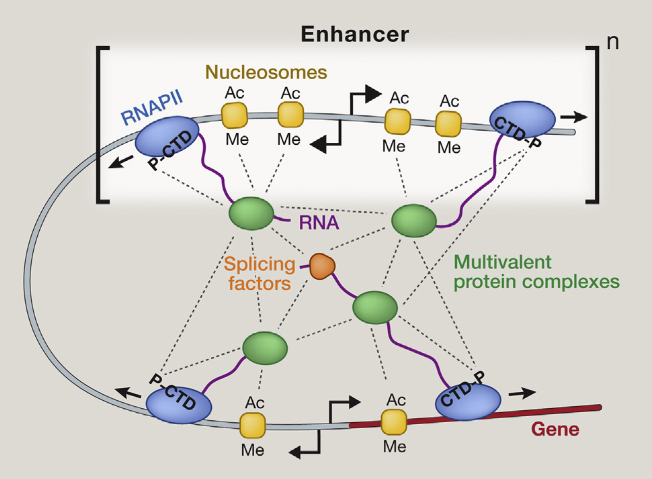
\includegraphics[width=8cm]{figure-5-6.png}
\end{figure}
\begin{figure}
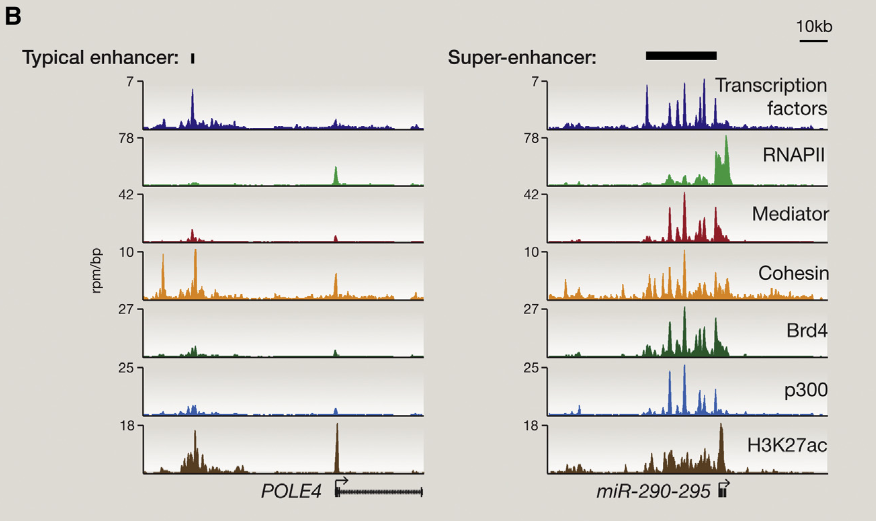
\includegraphics[width=9cm]{figure-5-2.png}
\end{figure}
\textit{Hnisz et al. A phase separation model of transcriptional control. Cell 2017}
\end{frame}


\begin{frame}{High-throughput imaging of GBP5 transcripts in single cells}
\begin{figure}
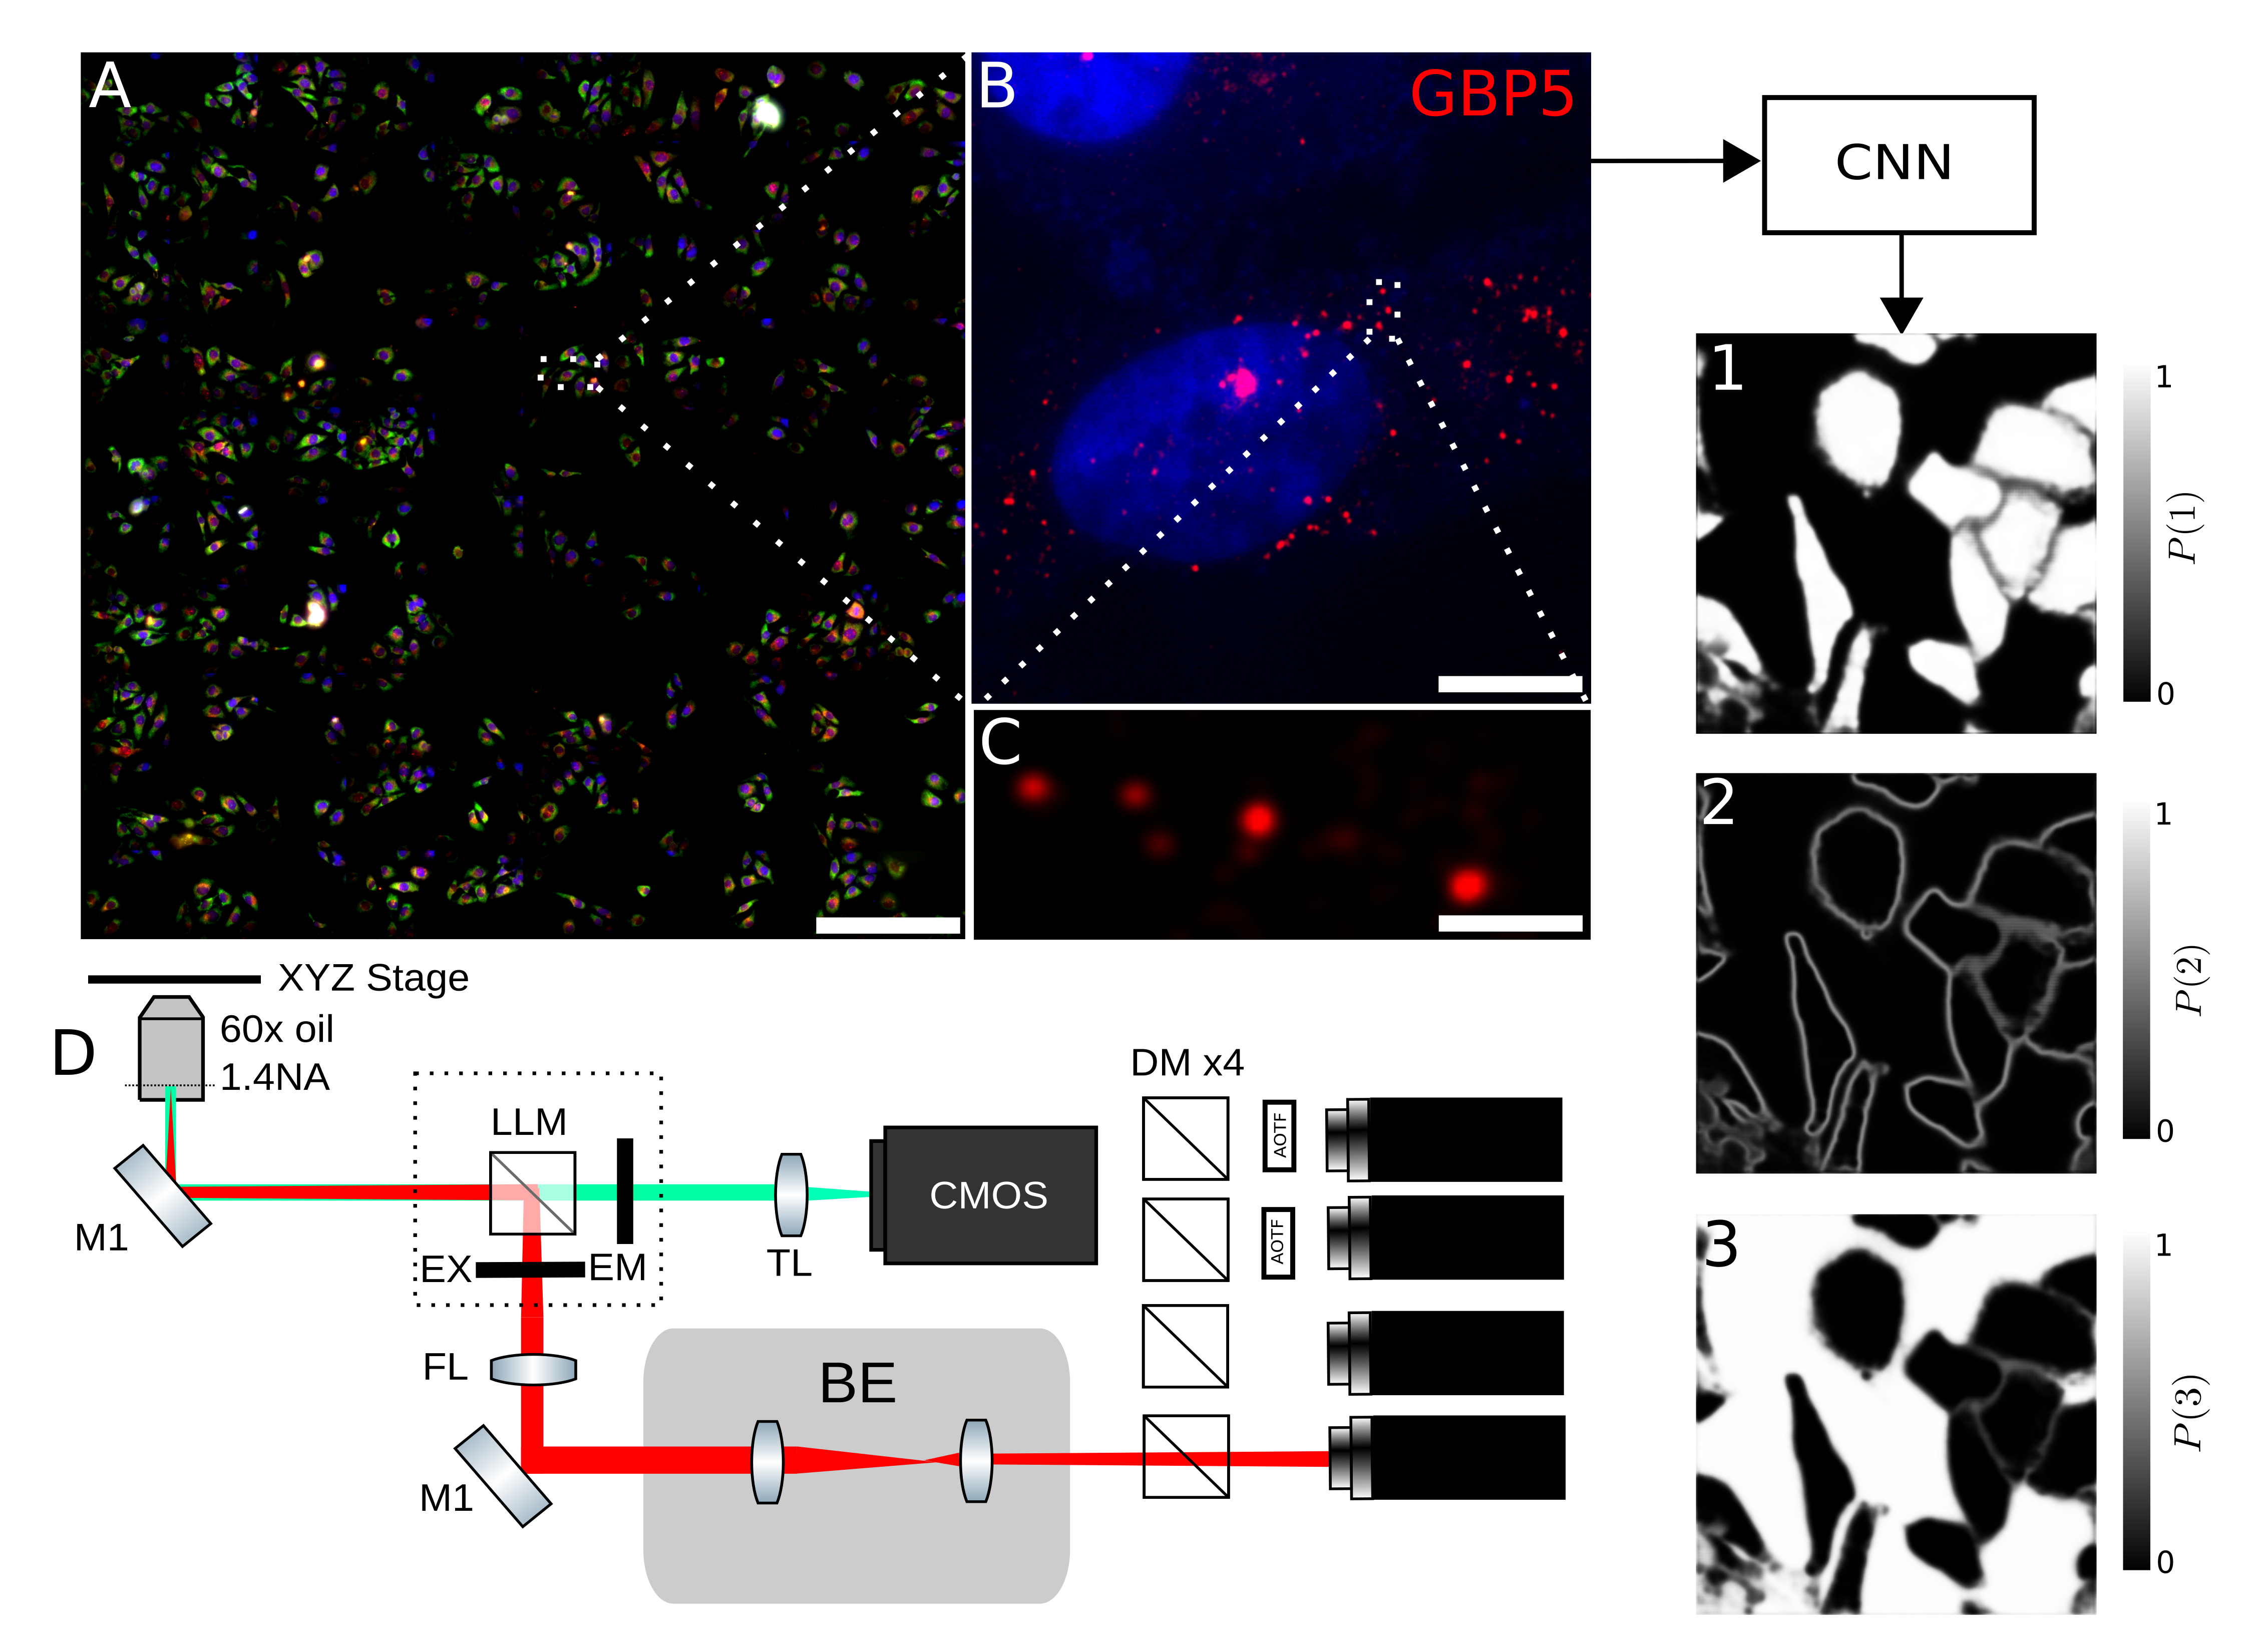
\includegraphics[width=11.5cm]{Figure-1.png}
\begin{itemize}
\item {\fontsize{8pt}{16.8pt}\selectfont (A) Large FOV three channel maximum intensity projection. Scalebar ~300um }
\item {\fontsize{8pt}{16.8pt}\selectfont (B)  GBP5 mRNAs. Scalebar ~10um }
\item {\fontsize{8pt}{16.8pt}\selectfont (C) Diffraction-limited image of GBP5 transcripts hybridized with 48 complementary fluorescent probes }
\item {\fontsize{8pt}{16.8pt}\selectfont (D) 4-color widefield microscope used for fluorescence imaging with a 60X Nikon oil-immersion objective.}
\item {\fontsize{8pt}{16.8pt}\selectfont (1-3) Single cell masks predicted by a convolutional neural network (CNN)}
\end{itemize}
\end{figure}
\end{frame}

\begin{frame}{Identification of GBP5 transcription sites}
\begin{figure}
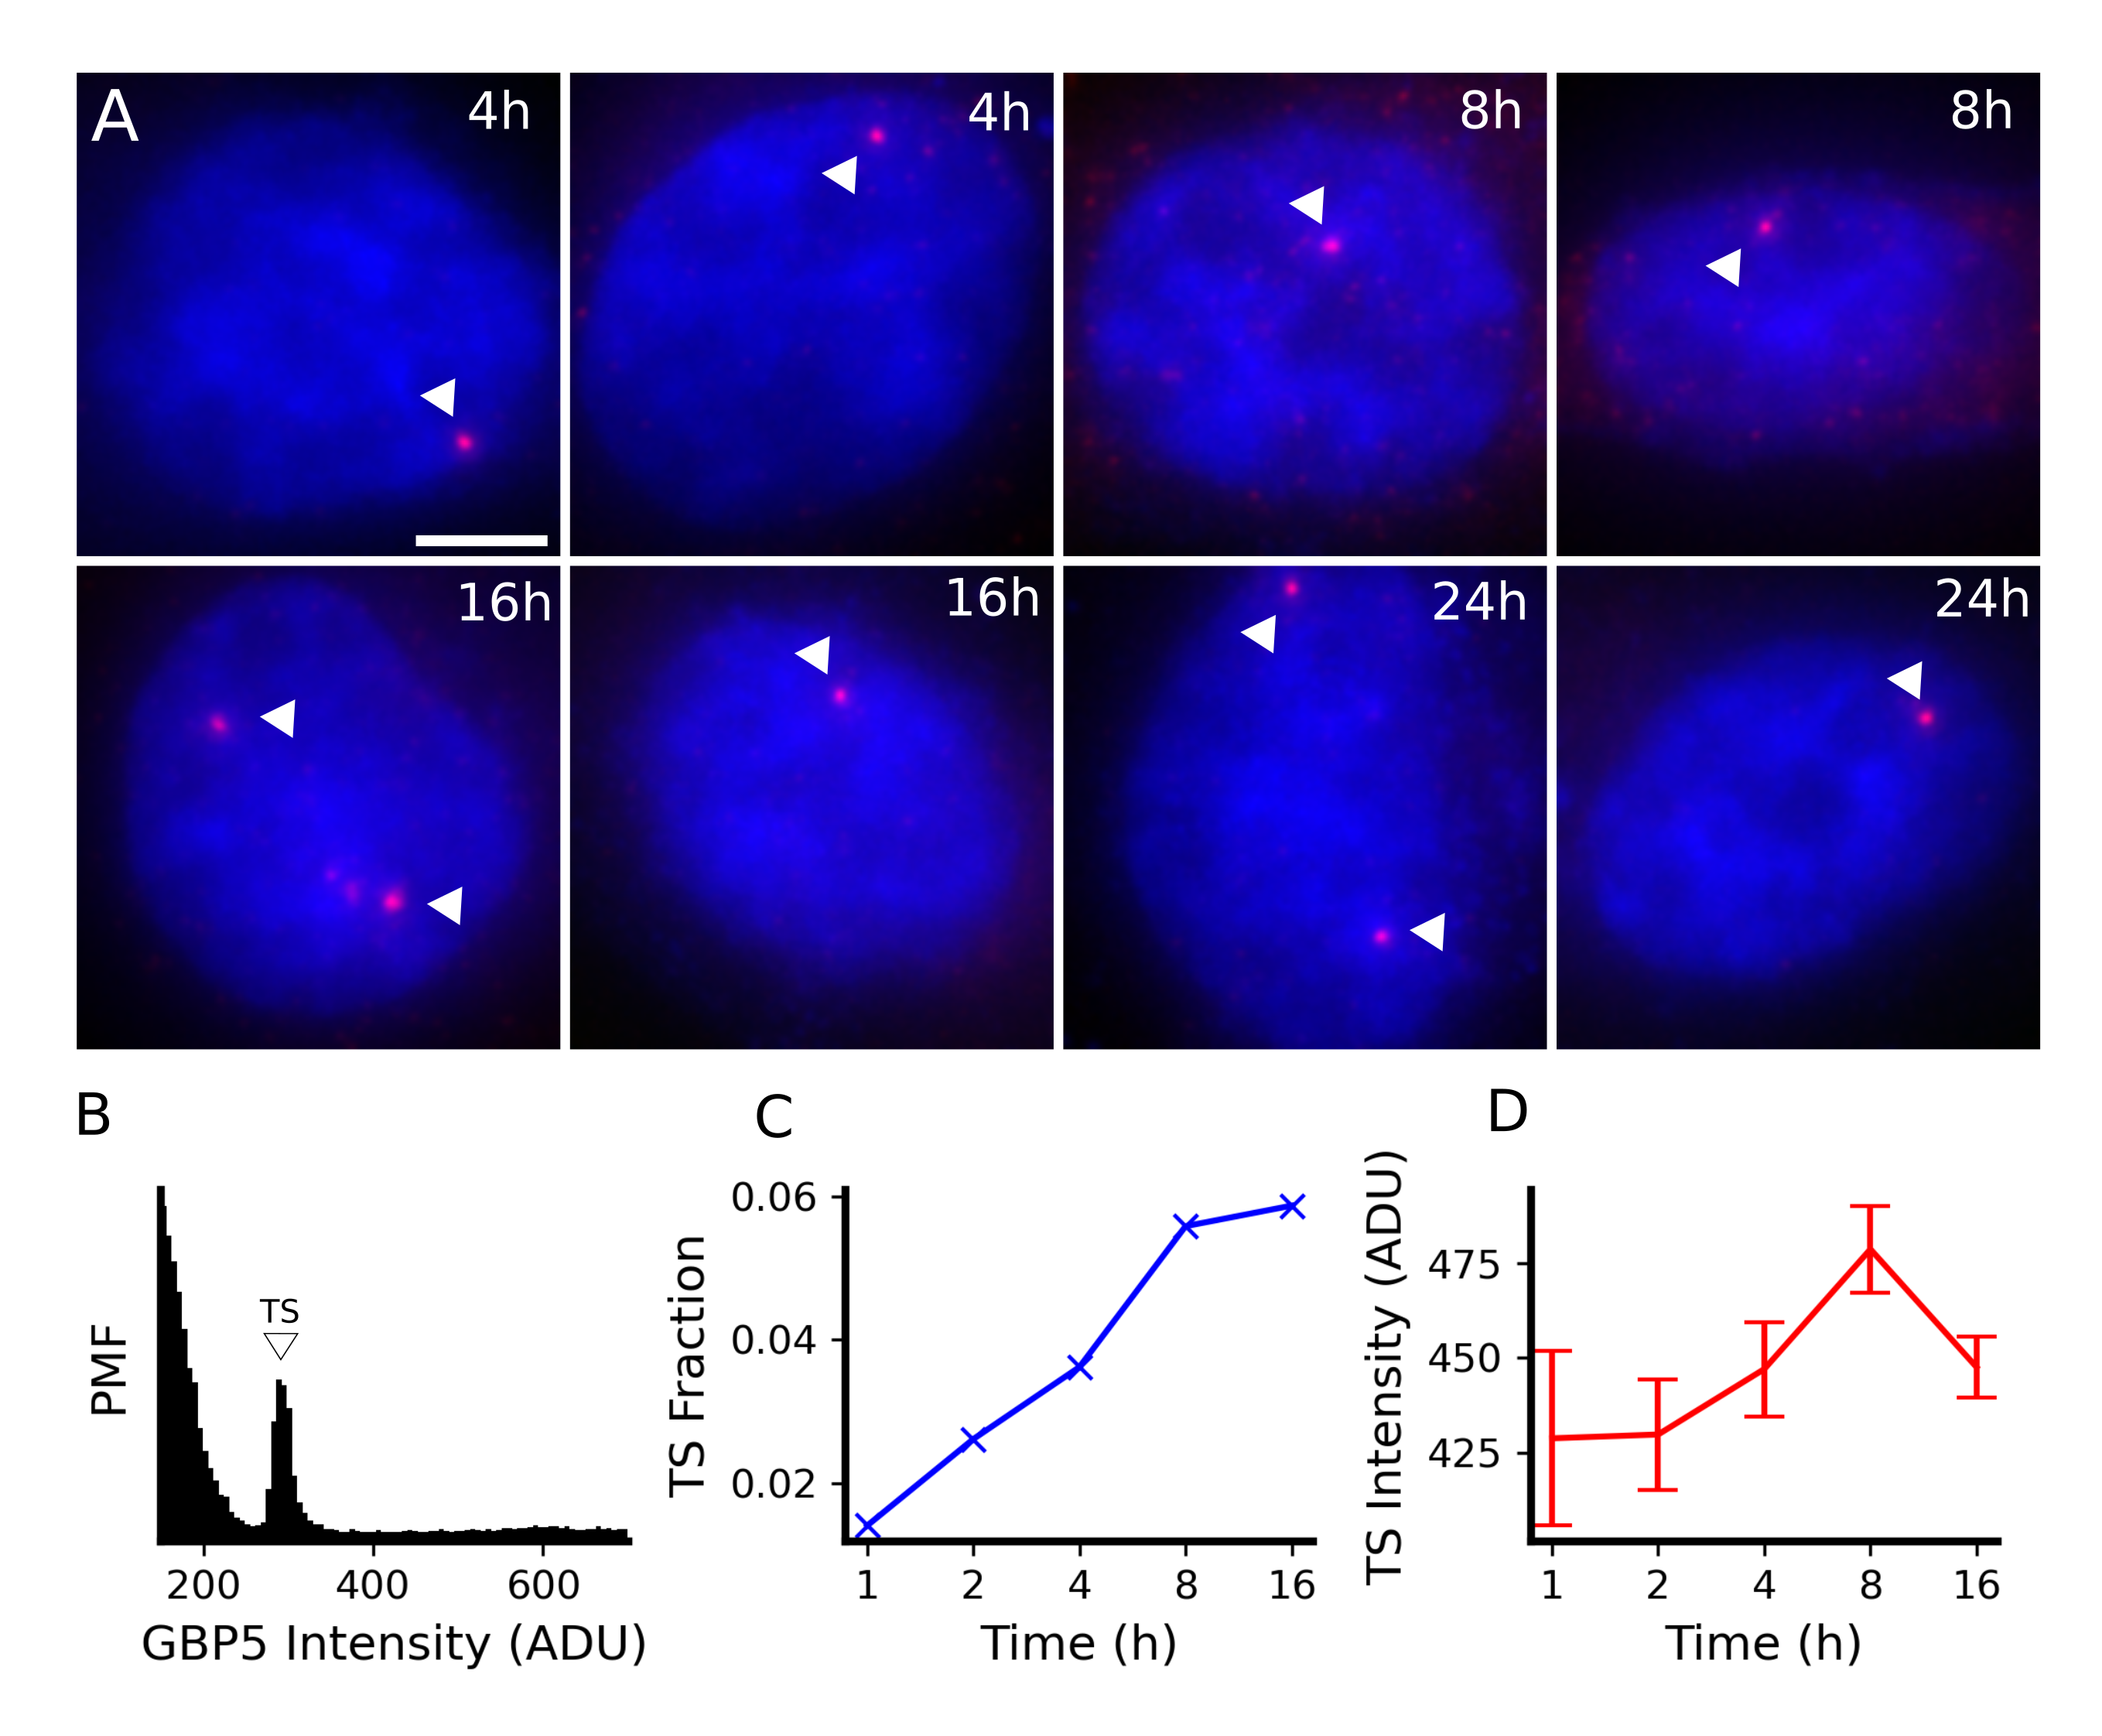
\includegraphics[width=10.5cm]{Figure-2.png}
\begin{itemize}
\item {\fontsize{8pt}{16.8pt}\selectfont (A) Putative transcription sites at 4h, 8h, 16h, and 24h after first exposure of HeLa cells to Interferon-gamma (50 ng/mL) }
\item {\fontsize{8pt}{16.8pt}\selectfont (B) Histogram of peak intensities of single GBP5 transcripts used to determine the criterion for transcription site classification. }
\item {\fontsize{8pt}{16.8pt}\selectfont (C)  The fraction of cells with at least one active transcription site as a function of time since first exposure to IFN-gamma }
\item {\fontsize{8pt}{16.8pt}\selectfont (D) Average intensity of putative transcription sites since first interferon exposure. Error bars represent standard errors}
\end{itemize}
\end{figure}
\end{frame}

\begin{frame}{High-throughput imaging of GBP5 transcripts in single cells}
\begin{figure}
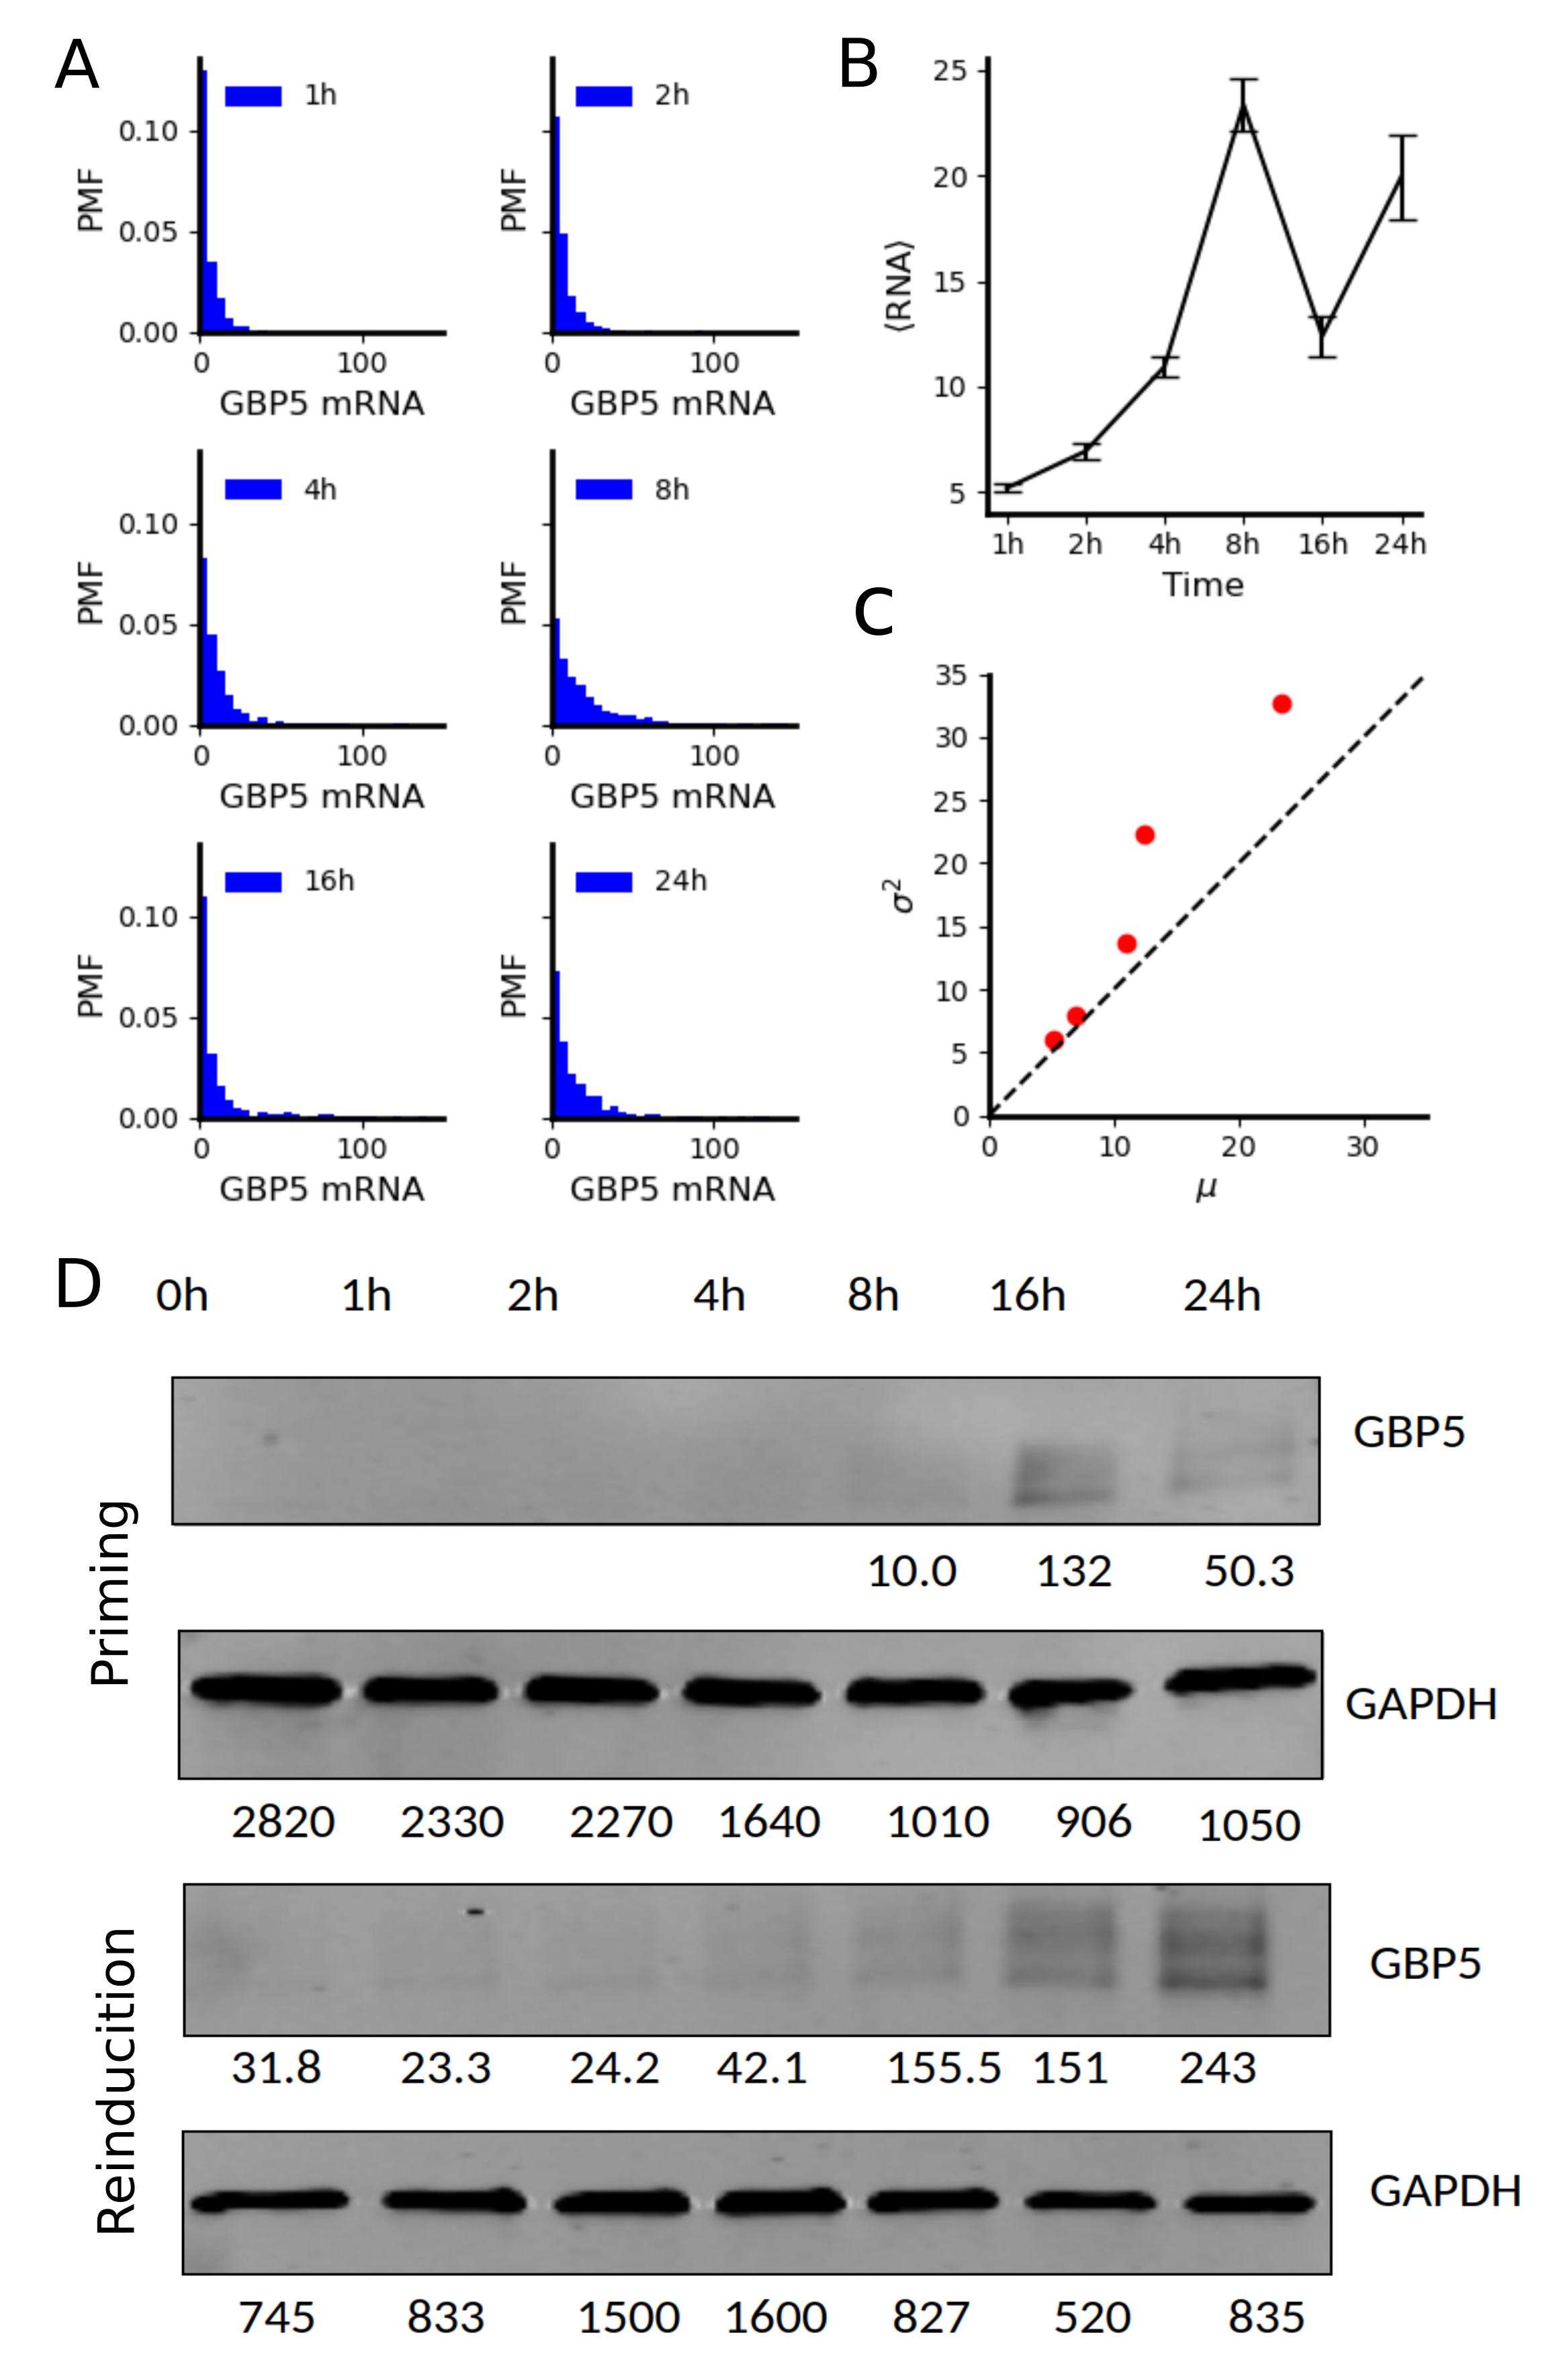
\includegraphics[width=8cm]{Figure-3.png}
\end{figure}
\end{frame}

\begin{frame}{RT-qPCR validation of GBP5 expression and identification of BRD4 as a potential transcription factor}
\begin{figure}
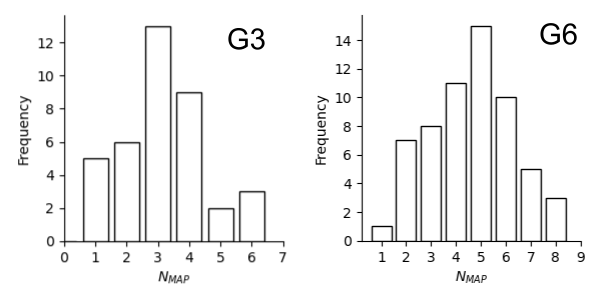
\includegraphics[width=10cm]{Figure-5.png}
\end{figure}
\begin{itemize}
\item Optimized sequential FISH + IF @ 8h after IFN-$\gamma$ exposure
\item Need to do analysis of GBP5 and BRD4 co-localization
\item Most papers use a DNA FISH probe to prove TS unequivocally
\item Can also try the JQ1 inhibitor
\end{itemize}

\end{frame}


\end{document}